\section{Task 1: Inductive Biases and Feature Representations}

\subsection{Experimental Setup}
% Brief 2-3 sentence overview of dataset (STL-10), architectures (ResNet-50, ViT-B/16,
% CLIP ViT-B/32 with a trained linear head and zero-shot prompts), 500-image balanced
% evaluation subset, and seed 6304.

\subsection{Model's Reliance on Shape, Texture, and Color}

\begin{table}[t]
  \caption{Top-1 accuracy (Acc, \%), change from each method's clean baseline ($\Delta$, pp) and prediction consistency (C, \%) on 500 STL-10 test images (seed 6304). $\dagger$: significant under a paired McNemar test with Holm correction ($p<0.05$). Hue rotation is $30^{\circ}$; patch shuffle uses a $4\times4$ grid.}
  \label{tab:task1_interventions}
  \centering
  \small
  \setlength{\tabcolsep}{4pt}
  \begin{tabular}{lccccccccccc}
    \toprule
    & \textbf{Clean} & \multicolumn{3}{c}{\textbf{Grayscale}} & \multicolumn{3}{c}{\textbf{Hue $30^{\circ}$}} & \multicolumn{3}{c}{\textbf{Patch shuffle}} \\
    \cmidrule(lr){2-2} \cmidrule(lr){3-5} \cmidrule(lr){6-8} \cmidrule(l){9-11}
    \textbf{Method} & Acc & Acc & $\Delta$ & C & Acc & $\Delta$ & C & Acc & $\Delta$ & C \\
    \midrule
    ResNet-50 head       & 97.8 & 96.4 & $-1.4$ & 97.0 & 96.2 & $-1.6$ & 97.0 & 90.0 & $-7.8^{\dagger}$  & 91.8 \\
    ViT-B/16 head        & 98.8 & 96.6 & $-2.2$ & 96.6 & 98.0 & $-0.8$ & 98.4 & 92.6 & $-6.2^{\dagger}$  & 92.8 \\
    CLIP ViT-B/32 head   & 97.8 & 95.4 & $-2.4$ & 95.6 & 97.8 & $+0.0$ & 97.4 & 84.0 & $-13.8^{\dagger}$ & 83.6 \\
    CLIP ViT-B/32 zero-shot & 96.8 & 94.4 & $-2.4^{\dagger}$ & 96.8 & 95.8 & $-1.0$ & 98.4 & 84.0 & $-12.8^{\dagger}$ & 84.4 \\
    \bottomrule
  \end{tabular}
\end{table}

\begin{figure}[t]
  \centering
  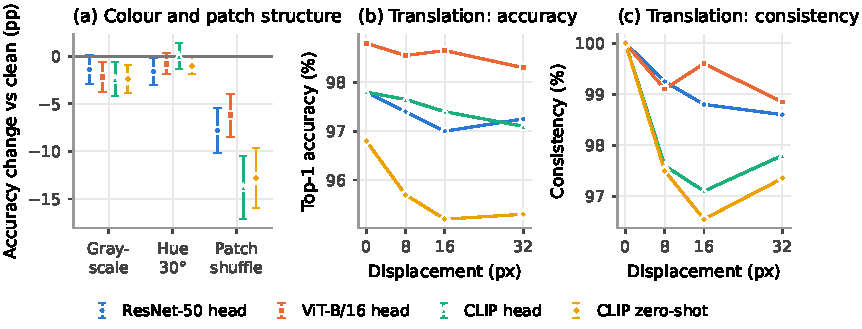
\includegraphics[width=\textwidth]{figures/task1/fig1_interventions.pdf}
  \caption{(a) Accuracy change from the clean baseline with 95\% confidence intervals; intervals crossing zero are within sampling noise. (b) Accuracy and (c) prediction consistency against translation distance, averaged over four directions ($N=500$).}
  \label{fig:task1_interventions}
\end{figure}

Model performance under interventions like color changes (greyscaling or hue modifications) showed no substantial drop in overall performance, suggesting that none of the models gave much importance to the color when making predictions. Removing color altogether cost between 1.4 and 2.4 points, and changing color impacted even less, from 0 to 1.6 points. Although, under the greyscale all four models broke more predictions than they managed to fix, only the zero-shot CLIP change was statistically more reliable.

When the texture of one class is pushed over the shape of another every models showed a strong inclination towards shape bias, with ResNet being the least biased towards shape and appearing to give some importance to texture as well as compared to the rest. Coverage of each model on the cue conflicts gives a different base for these percentages. For ResNet the shape bias is computed from 160 predictions, while for the others from about 180. A lower coverage means the model committed to a cue on fewer images. The models, ViT, the CLIP head, and zero-shot CLIP, predicted a third class on only 17 to 20 of the 200 conflicts, while ResNet did so on 40. Thus, ResNet's shape bias is measured less precisely than the others (Table~\ref{tab:task1_shape_bias}). However it cannot claimed that ResNet's lower coverage follows from its greater reliance on texture or from some other weakness, since a third-class prediction only shows that neither cue won, not which cue caused it.

For the three trained heads (ResNet $+14.5$, CLIP head $+12.0$, ViT $+7.0$ points) the texture class rose into the top two of the ranked class scores more often under conflict than on the clean content image, so texture does influence their scores even though shape still dominates the final decision; zero-shot CLIP showed no such reliable movement.

\begin{table}[t]
  \caption{Cue-conflict decisions on 200 AdaIN conflict images ($\alpha=0.7$). Shape bias $=N_{\text{shape}}/(N_{\text{shape}}+N_{\text{texture}})$; coverage $=(N_{\text{shape}}+N_{\text{texture}})/200$. Brackets: 95\% intervals (bootstrap for shape bias, Wilson for coverage).}
  \label{tab:task1_shape_bias}
  \centering
  \footnotesize
  \setlength{\tabcolsep}{4pt}
  \begin{tabular}{lccccrr}
    \toprule
    \textbf{Method} & \textbf{Shape} & \textbf{Texture} & \textbf{Other} & \textbf{Decisions} & \textbf{Shape bias (\%)} & \textbf{Coverage (\%)} \\
    \midrule
    ResNet-50 head       & 139 & 21 & 40 & 160 & 86.9 [81.4,\,91.9] & 80.0 [73.9,\,85.0] \\
    ViT-B/16 head        & 179 & 4  & 17 & 183 & 97.8 [95.6,\,99.5] & 91.5 [86.8,\,94.6] \\
    CLIP head            & 171 & 11 & 18 & 182 & 94.0 [90.2,\,97.2] & 91.0 [86.2,\,94.2] \\
    CLIP zero-shot       & 172 & 8  & 20 & 180 & 95.6 [92.2,\,98.3] & 90.0 [85.1,\,93.4] \\
    \bottomrule
  \end{tabular}
\end{table}

\begin{figure}[t]
  \centering
  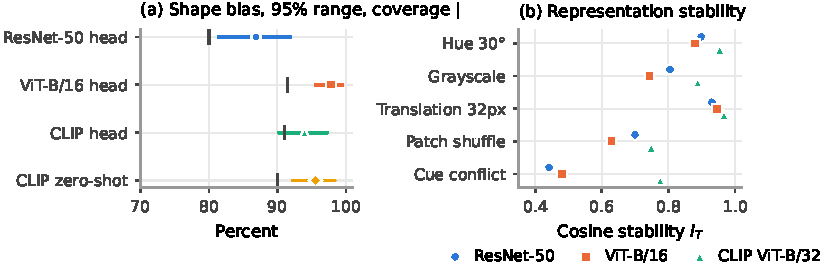
\includegraphics[width=\textwidth]{figures/task1/fig2_cue_and_representation.pdf}
  \caption{(a) Shape bias with 95\% interval, and coverage ($|$), per method. (b) Cosine stability $I_T$ between clean and transformed features per backbone (1 = unchanged); translation averages four 32-pixel shifts. The two CLIP methods share one backbone.}
  \label{fig:task1_cue_representation}
\end{figure}

\begin{figure}[t]
  \centering
  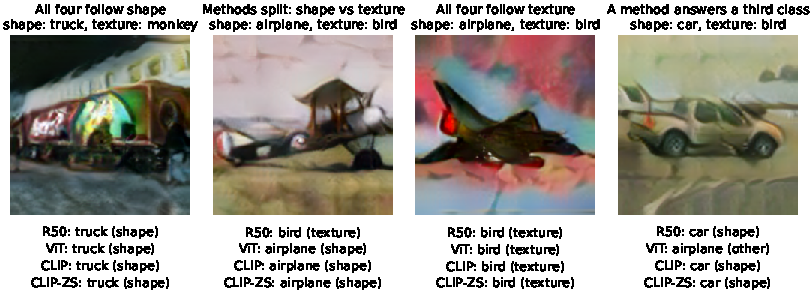
\includegraphics[width=\textwidth]{figures/task1/fig3_cue_examples_compact.pdf}
  \caption{One seeded cue-conflict example per decision pattern (out of 200: all shape 126, split 24, all texture 2, a third class 55), with each method's prediction and whether it follows shape, texture or neither.}
  \label{fig:task1_cue_examples}
\end{figure}

\subsection{Spatial and Positional Invariance}

Models show almost no drop in accuracy and performance with translations. Out of the 48 translation tests (8, 16, and 32 pixels across four directions and four methods), only 8 resulted in 10 or more predictions flipping to negative, with a maximum of 16 (zero-shot CLIP at 16 pixels left), and 7 of these 8 cases belong to zero-shot CLIP. The confidence intervals permit a performance decline of up to approximately 4 points, thus ruling out major degradation from translation while leaving smaller losses possible.

All four drops were statistically reliable, with ResNet and ViT models' performance declining by 6.2 to 7.8 points, where ResNet failed on 39 correct baseline predictions and was unable to correct a single incorrect baseline prediction. The CLIP models appeared to be hit the worst, with the CLIP head breaking 75 predictions while fixing only 6, and overall performance decreasing by 12.8 to 13.8 points. This difference is reliable, as both CLIP methods lost significantly more than ResNet and ViT.

The variation in model performance can be attributed to the changes introduced by each intervention. During the translation interventions, most of the global image and shape structure is preserved. Models still have access to enough global representation, evident from the feature similarity between 0.93 and 0.98 when comparing baseline and translated images, and they therefore retain their accuracy and consistency. This changes substantially with patch shuffling, which moves the patches around and destroys the global spatial arrangement: representational similarity falls to between 0.63 and 0.75, and all models lose accuracy. The correspondence holds when comparing the two interventions, but not when comparing models, since CLIP keeps the highest similarity under shuffling (0.748) while losing the most accuracy ($-13.8$ points), and ViT has the lowest similarity (0.629) with the smallest loss ($-6.2$ points). Furthermore, local features retain significant diagnostic value independently: since patch shuffling keeps every pixel and local texture within each block intact, the models maintain an accuracy of 84.0\% to 92.6\% despite the loss of spatial layout---substantially above chance level. This demonstrates that local texture information sustains the majority of the classification performance, whereas global structure provides the final 6.2 to 13.8 percentage points.

\subsection{Representation Space Analysis}

For all models, feature representation similarity remained quite stable across translations. For color interventions it drops marginally. However, a substantial decline is observed for patch shuffling ViT(0.63) , ResNet(0.70) , CLIP(0.75). Cue conflicts caused the sharpest drop of all, ResNet(0.44), ViT(0.48), but CLIP managed a good performance of 0.78 points.

On translation interventions the features barely moved, (stayed 0.93 $\sim$ 0.98), and accuracy remains stable. The clearest divergence appears with the cue conflicts, where ResNet's representation moves the furthest of all (dropping to 0.442), while its predictions change only slightly, since 139 of 200 still follow the shape class. A possible explanation is that cosine similarity measures how far the representation moved, not what it still contains, so a large movement does not necessarily remove the information the classifier relies on. In these cases, prediction stability and representation stability come apart.

Another interesting finding is observed for ViT on the cue conflicts, where the similarity is 0.505 for stable predictions against 0.264 for flipped ones, showing that the images whose predictions flipped had moved further than those that held. However, under patch shuffling that gap nearly vanishes (0.014 for ResNet), so feature movement barely explains which predictions broke there. Representation change and prediction change therefore agree within a condition, while diverging across conditions.

CLIP lost the most accuracy under shuffling ($-13.8$ points), while ViT moved furthest (0.629 under shuffling) and lost the least ($-6.2$ points).

\begin{figure}[t]
  \centering
  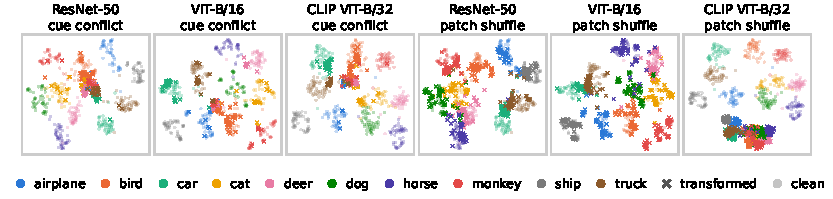
\includegraphics[width=\textwidth]{figures/task1/fig4_tsne_strip.pdf}
  \caption{Joint t-SNE of clean (dots) and transformed (crosses) features per backbone, coloured by class (content class for cue conflicts); coordinates are comparable only within a backbone. In CLIP's patch-shuffle panel the transformed points form a separate cluster although 84.0\% are still classified correctly.}
  \label{fig:task1_tsne}
\end{figure}

CLIP vs CLIP Zero-Shot predicted same class for the same image and they share similar accuracy on the baseline, translations and colour changes. The visible differences come from patch shuffle and cue conflicts. Under patch shuffle the accuracy numbers of the two are identical (84.0\%), yet their agreement on the predicted class drops to 88.2\%, meaning they disagreed on 59 of 500 images, with 22 correct only for the head and 22 correct only for zero-shot. Under cue conflicts agreement is similarly low at 88.0\%, and the texture-rank analysis shows that the transferred texture reliably raised the texture class in the head's top two ($+12.0$ points) but not in zero-shot's ($+0.5$, not reliable). With same backbone embeddings, the two decision rules read those same representations differently, and the trained head is the more texture-sensitive of the two.

\subsection{Architecture and Observation Relationships}

The models differ across their architecture, pretraining data, supervision, and capacity. Such cross-model differences are therefore confounded and cannot be attributed to architecture alone.

Across this experimentation, the one causal claim that can be made about the decision rule comes from comparing CLIP with a trained linear head against zero-shot CLIP. Since both share the same frozen backbone, the same pretraining and identical image embeddings, the observed differences must be driven by the decision rule rather than the representation, as highlighted in their comparison earlier.

A partial architectural link can be drawn between ResNet and ViT. Both were pretrained on the same dataset (ImageNet-1k) with the same supervision (class labels), so data and supervision are held constant. ResNet's reliably lower shape bias (86.9\% vs 97.8\%) and lower coverage (80.0\% vs 91.5\%, driven by 40 third-class predictions concentrated in cases like monkey-to-truck and deer-to-car) indicate a relatively greater reliance on texture than the other three, which is consistent with the convolutional inductive bias reported in the literature. However, the two models also differ in capacity (25M vs 87M parameters) and training recipe (the \texttt{IMAGENET1K\_V2} ResNet weights use heavier augmentation), so architecture cannot be isolated as the cause. The shape bias built into our conflict set raises the absolute level for every method equally, so it explains the high values overall but not the difference between models.

Conversely, CLIP's substantially larger accuracy degradation under patch shuffle ($-12.8$ to $-13.8$ points, compared with $-6.2$ to $-7.8$ for ViT and ResNet) cannot be assigned to architecture, since CLIP differs from ViT in patch size (32 px vs 16 px), supervision (multimodal contrastive) and pretraining scale (400M web pairs) at the same time. The fact that both CLIP variants suffer equally does show that the effect comes from the representation rather than the decision rule.

Definitively isolating these underlying mechanisms would require controlled ablations holding non-architectural factors fixed, such as comparing a supervised ViT-B/16 directly against a CLIP-trained ViT-B/16, or training CNN and Transformer backbones under identical dataset sizes, augmentations, and optimisation recipes.
